






\subsection{image captioning}

Image captioning is an extensively researched field where visual-grounding is at the  center of its focus. The methods of image captioning provide insights helpful for tasks that combine vision an language. In this section we review two main methods used in image captioning,feature extraction and attention mechanisms.   


\subsubsection{Feature extraction}

Feature extraction methods can be divided into two main groups. The first group relies on statistical language models(described in the previous section as transparent function). The second group relies on encoder-decoder neural network model that deep extracts features.\cite{Imagecap}

\paragraph{Encoder-Decoder(CNN-RNN)}



Convulutional neural networks are at the core of feature extraction methods. CNN applications, nonetheless, take a vital role in many computer vision tasks. We see CNN and its modified models (such as recurrent-CNN) used in tasks as object recognition \cite{liang2015recurrent} \cite{objdet} \cite{Ren2015FasterRT} , image classification \cite{simonyan2014very} \cite{imclassfication},and  semantic segmentation \cite{hariharan2015hypercolumns} \cite{imseg}. 

A main reason for using CNN for image processing  is its ability to reduce the high dimensionality of images. Image features contain large sizes represented in pixels which would require large number of parameters to train. CNN reduces the dimensions of an image by learning how to process a matrix from a large window such as 250x250 pixels into a smaller one as 25x25. Through computing the convolution values of the image matrices and executing pooling computations, this process reduces the image into a smaller representation. The latter reduces the computational load and helps in processing and classifying the images faster.   


The encoder-decoder caption generation has a CNN encoder and an RNN decoder.\cite{vinyals2015tell} is an example of an end-to-end neural captioon generation model. In the neural model the CNN process the image features, and the last hidden layer passed to an RNN to generate a description. This method is a sequence modeling that is similar to machine translation. This means that image features are translated into words. The sequence is predicted by finding the probability of a certain description from a corpora given the features of an image. 

RNN are known to be used widely in language technology applications. Rnn is used , for example in  text-to-speech \cite{arik2017deep} and  machine-translation \cite{cho2014learning},\cite{Wu2016GooglesNM}. The advantage that the RNN gives to these tasks is that the output size is not fixed and that each output depends on the previous one. Such an incremental-sequence prediction is suitable for sentence predictions in respect to word dependency.  

RNNs have a issue of vanishing gradient-descent. The gradient descent is an optimization algorithm that minimizes the error calculated in the loss function. Optimization, in brief description, is important for the learning process. It updates the model's parameters which determines the  direction taken in the next time-step. This information is calculated given the input-output and the values of the parameters from the previous time-stamps. The gradients is reduced at every step due the value deductions in the activation function. When the gradient is reduced to almost zero value, it will be updating the parameters with no useful values, and therefore, learning seizes to improve. 

Long-Short-Memory network (LSTM)  provides a good alternative for avoiding the disappearing gradient. The gradient in RNNS vanishes in long sequences where the gradient keeps reducing. The architecture of the LSTM allows it to keep information stored for very long sequences. The latter gives it the ability to control the values of the gradient by updating it with information stored in the 'forget gate' form previous steps, preventing the gradient from vanishing.  



\paragraph{Feature extraction- statistical language model}

Statistical language model, as in \cite{fang2015captions}, generate descriptions in three stages. First it detects words in an image using a convolutional neural network (CNN) for extracting image features. The incorporation of language at this stage happens using multi-instance learning(MIT)\cite{zhang2005multiple}. The second stage, the statistical language model detects the most likely sentence to make of the words from a pre-defined corpus. In the third stage the sentences undergoes a re-ranking stage where the sentences are combined to generate captions. 


%\subsubsection{Attention-mechanisms}



\subsection{Dialogue and VQA}

In this section of the text we discuss the capabilities of computers to exhibit more intelligent behaviour. Image-captioning and its methods showed an insight to how much computers could see and understand what its seeing. However, acquiring language in the visual world would require computers to be able to communicate what it sees. Otherwise, in order to say that a computer is visually or linguistically intelligent one should imagine the computer having to pass the Turing test in a visual surrounding. 

Researchers attempt to improve systems that are capable to hold a dialogue with a visual content.\cite{das2017visual} trains a system in  encoder-decoder model on a data set of 2 pairs dialogue with an image content.\cite{Skoaj2011ASF} trains a system on learning concepts with visual content in an interactive-learning approach. In the similar context of improving systems that are capable of having more natural interactions, we see example in \cite{Lin2014VisualSS} of a VideoQA. 

To make a true statement about the computer's capability to engage in a visual dialogue, it must be first ensured that the computer actually understands the questions being asked to it. Otherwise, dialogue is very complex with many elements determining its succession. In a dialogue with visual content, the computer must, furthermore, understand the questions within their visual context. It is reasonable that we see increasing research on "Visual Question Answering" and less on visual dialogue as a whole. Improvements in VQA intuitively means that we are moving closer in the direction of having an interaction with a computer in a visual dialogue.  


 \cite{VQA} is the first notable data-set published for Visual Question answering (VQA). The data-set consist of open-ended and free-form questions. The data contains 250,207 images from MS COCO \cite{lin2015microsoft} and other abstract scenes.The question types in the dataset require a range of different capabilities such as common-sense reasoning, knowledge-based reasoning, object-detection and active recognition.
 
 Data-sets that use MS COCO scenes such as \cite{gao2015talking}, \cite{yu2015visual} in addition to \cite{VQA} used human workers to write the texts for the scenes. Other data-sets are generated automatically such as \cite{ren2015exploring}. 


\cite{zhu2016visual7w} introduces a  unique QA data-set. The Visual7W consist of questions about an image with objects marked with regions in the image. Object grounding with image region introduced in \cite{krishna2016visual} contains the largest data-set with regions for both VQA and Image-captioning. Object-region approach is intended to improve visual grounding, by marking the regions of the image that the strings refer to.

restricted visual Turing test to evaluate visual understanding. The DAQUAR dataset is the first toy-sized QA benchmark built upon indoor scene RGB-D images. Most of the

\subsection{Embodied Question Answering}

\begin{figure}[H]
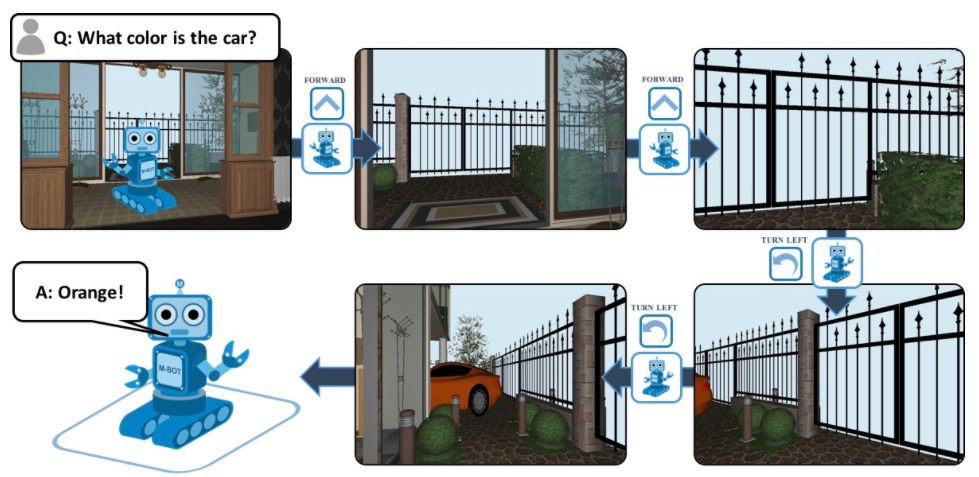
\includegraphics[scale=0.4]{images/EmbodiedQuestionAnswering.png}
\label{fig:EQA}
\caption{The Robot is asked a question at a start position. It needs to look a round, collect information and decide on the next step to take. When it recognizes the car it stops and processes the scene to answer the question }
\end{figure}. 

Embodied Question Answering is a new interactive task presented as one of the tasks within the Habitat Platform (\cite{embodiedqa}). \footnote{Link to the official page of EQA. It includes also other published papers about the task \url{https://embodiedqa.org/}.} \footnote{Github link to the Habitat Platform. Information and code about EQA and the other tasks within Habitat can be found there \url{https://github.com/facebookresearch/habitat-lab}.} The idea of the task is to allocate an agent at a random position in an  3D environment and ask it a question. To answer the question, the agent must intelligently explore the environment, collect information, and successfully navigate to the entity in question. EQA system navigates based on common reasoning, through an egocentric view, more or less imitating humans, it should be able to answer itself the common questions of “where am I?”, “where to go next?” and if asked a question about the car, as seen in \ref{fig:EQA}, it should be able to reason that cars are usually situated outside or in the garage and look for the exit. Once it navigates successfully to a point where it recognizes the car, the robot should stop and answer the question.  


\begin{figure}[H]
\centering
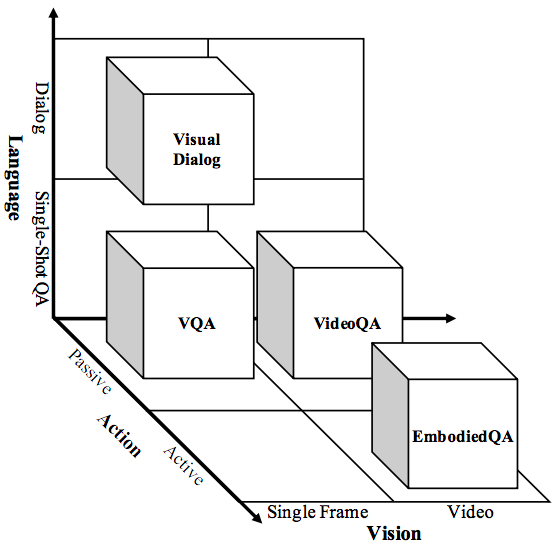
\includegraphics[scale=0.3]{images/Vision-language.png}
\caption{EQA in relation to other vision\&language multi-modalities}
\label{fig:multimodal}
\end{figure}.


In figure \ref{fig:multimodal} we see where EQA stands in relation to other vision-and-langiage multi-modalities discussed earlier. In the language domain we see single-shot and  dialogue. VQA is a typical example of a single shot interaction, where the system is designed to take a single shot question and a visual scene and output an answer. On the other side of the language domain (dialogue) we see Visual Dialogue where the interaction within a visual context is continuous. On the vision domain we see that VQA Visual dialogue  are distinguished from VedioQA and EQA by the visual input type. The robot in EQA is continuously moving while navigating so it inputs the vision similar to videos. Finally, EQA is distinguished from the rest of the multi-modalities on the action domain by being active. Hence, action here refers to executions of commands in a physical space. EQA is action-active by its navigational functionality. The rest of modalities are passive with no functionalities of physical action execution. 


The novelty of this system is that it presumably solves a problem of navigating and performing tasks in unseen environments. Many of the earlier studies that deal with navigation such as \cite{kruijff2007situated}\cite{lauria2001training} require the system to have a localized map of the environment in order to be able to navigate in it. The problem of localization in robotic navigation is known as Simultaneous Localization and Map Building(SLAM). SLAM is a problem where a robot should be able to  map an unknown environment without a GPS or local map. Simultaneous localization is when a robot discover its surrounding and simultaneously construct a map while aware of its changing location. This means that the robot should extract information from its surrounding and learn the map as it goes \cite{grisetti2010tutorial} \cite{938381} \cite{8482266}. 


The answering system in the robot consist of two core components. The first is navigation, and the second is Visual Question Answering. In principle the task should be preformed in conjunction between the Nav and the VQA model. The navigation should lead the robot to a correct view-point then freeze its move, the VQA model, should then take static image frames of the scene, from the view point where the Nav stopped, and answer the question. 
However, the design of the system allows it to exclusively perform either navigation or visual question answering on baseline models. The ability to train and evaluate either of the modules is made possible due to two different training setups.

\subsubsection{Training setups}

The first setup is a connected system with training in Reinforcement Learning setup. The training of the robot in RL happens on the basis of answer-base evaluation. The robot is rewarded if the it completes the whole task using the two components connected.  The basis of evaluation in the RL setup is the answer prediction. The system is rewarded if it answers the question correctly, and to answer the question correctly it needs to navigate to the right place and stop at good view-postion so that the VQA system could have a relative and informative visual scene in order to answer the question.However, the researches in \cite{embodiedqa} elaborate that the system preforms poorly when trained combined in RL. The navigation in RL setup tends to position itself inaccurately at the stop-goal which leads to passing distorted images to the VQA model."Noisy or absent views"  would confuse the question-answering model \cite{embodiedqa}. For the mentioned reason, there are no available RL-based system available for developers. 

The second setup is a system with the Nav and VQA components trained separately and differently. The navigation is trained in 'Imitation Learning' setup and  VQA is trained  in Supervised Learning.\cite{hussein2017imitation} describes Imitation Learning as learning with a teacher, where a robotic system has to mimic the steps taken by its tutor. Imitation Learning is considered an effective solution, in particular, for navigational problems as its step-to-step learning restricts the freedom of systems; We see IL popular, for example, in navigational systems of ground vehicles \cite{silver2008high}. The available Nav and VQA models, that are available for training and evaluation in the habitat platform, are the baseline models.  The details of the training and the data used in each component will be described in more details in the coming sections. A main point we are trying to convey here is that the answering system that is being researched is a one with  Nav and VQA  components trained and tested differently. 

\subsubsection{Data} 

The data-set for the EQA task is called "EQA-MP3D" and it is a synthetic data-set generated automatically.\footnote{The data-set can be found on the github page of the Habitat Platform, attached in the main page in the section 'Task Datasets' \url{https://github.com/facebookresearch/habitat-lab}.}  The EQA-MP3D task data-set is applicable for navigation and VQA, meaning that training the navigation and VQA uses the same data-set.  We refer to each question-answer in the EQA data-set as an "Episode", because each QA sample includes a complete trainable navigation episode. We could describe the QA episode as a function that is executed in a 3D environment to yield an answer. 

The 3D environments used in the task are indoor environments from the Matterport 3D(MP3D) data-set \cite{eqa_matterport}.\footnote{ The github reop of the Matterport 3D \url{https://github.com/niessner/Matterport}.} The MP3D is 3D constructed scenes data-set which contains 90 segmented houses. The EQA trains the robot in 57 MP3D environments and test the robot in 10 other unseen MP3D environments.  

\paragraph{Data in the Navigation training}

In each QA episode, the information that is mainly used for navigation is a question,  an ID for the 3D Environment, a unique starting position,a destination-goal , and a path to the destination. The mentioned navigational information, excluding environment ID and question,  are all represented in frequencies of coordinates. The starting position indicates were the agent should be spawned relative to the given environment.  The path is the shortest path that the agent would take to reach the goal, which consists of steps and rotations that the agent. The shortest path is data used for Imitation Learning as the robots has to imitate the steps found in it. The goal is the stop point that marks the end of the episode. The stop point of the navigation is the view point of the entity in question 

\paragraph{Data in the VQA training}

In each QA episode, the information used for training the VQA model is an ID for the 3D Environment, a question, ground truth answer, and the position of view. The mentioned information is automatically taken ,in a code part of the Habitat platform, and reconstructed into conventional  VQA data-set, QA pair and a visual scene. The visual scenes are extracted using the view positions given in each QA episode in the corresponding 3D environment represented by the ID. 

\begin{figure}[H]
\centering
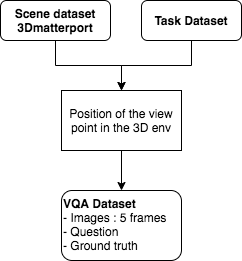
\includegraphics[scale=0.5]{images/VQAConstruct.png}
\caption{Locations of view points of the entity taken from an EQA episode to extract a visual scene. The visual scene is then constructed with a QA pair to form a VQA sample of 5 frames of images, question and ground truth }
\label{fig:vqaconstruct}
\end{figure}.

The extracted scenes for VQA consist of 5 frames images taken from the view point where the navigator is supposed to stop. In figure \ref{vqaconstruct} we see an illustration of the structuring of the VQA data-set using the EQA task data-set (EQA-MP3D) and the scenes in Matterport 3D. The resulted VQA for VQA training is a Quesiton-Answer pair with a visual scene. 

\paragraph{Data-set size \& Question types}

The question-answer data-set contains three types of questions. Each question-type is generated in a string template.The templates are as the following:

\textbf{- color\_room} template: "what color is <obj> in  <room>?": In these questions the agent needs to find the room in question and look for the object and answer the question. For the agent's to be successful at reaching its target, it needs to know the difference between rooms, and objects, as by implicitly recognizing that a certain room is a living-room, not a bathroom and such.  

\textbf{- color} template: "what color is <obj>". The difference between "color" type and "color room" is that no room is specified in the "color" type of question. In "color" type the agent needs to figure out where to look by itself. For example, "what color is the fridge?", the robot needs to implicitly figure that the fridges are usually in the kitchen and navigate to the kitchen to answer the question. In other cases, the object could be in the vicinity of the robot's starting point, so that it all it needs to do is to look around. 

\textbf{- location} template: "What <room> is the <obj> located in". 

In EQA-MP3D, each object in a question is unique to the room. The latter means that for an object to be selected for a question, there need to be only one instance of that object existent in the room. The reason for this is to avoid ambiguity, and not to confuse the agent if there happen to be more instances of the same object in the room. 

There is a total 11496 question-episodes in the train split and 1950 question-episodes in the val split. As seen in figure \ref{fig:questioncount},in the train split there are 1830 episodes of  "color" type, 8031 episodes of "color room"  and "1635" of location type. For the validation split there are 1335 "color room" questions, 345 "color" questions, and 270 "location" questions. 


\begin{figure}[H]
\centering
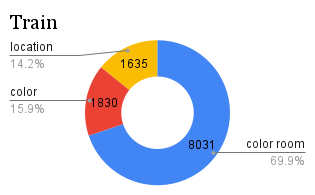
\includegraphics[scale=0.45]{images/Train.png}
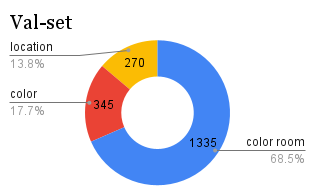
\includegraphics[scale=0.45]{images/Val-set.png}
\caption{Number of question-answers represented by their types in the Train and Validation set}
\label{fig:questioncount}
\end{figure}

The number of unique question-answers, however, is different from the number of episodes. A unique question-answer as a question-answer of the same strings and visual scene. For every unique question-answer and goal (scene) there is 15 different starting positions and shortest paths for the robot to train on for navigation. This means every unique QA in VQA is repeated 15 times. For example, in the validation set the number of unique questions (same QA and goal-scene) of "color" type  is 23, we multiply it with 15 (the number of starting positions for every unique goal) and we get 345, the number of episodes for "color" type in val-set as seen \ref{fig:questioncount}. In the train set, the number of unique visual-question-answer for "color\_room" is 536, for "color" is 122, for "location" is 109. In the val set, the number  of unique visual-question-answer for "color\_room" is 89, for "color" is 23, for "location" is 18. 


\paragraph{Data Bias}

In all color questions (color \& color\_room) in the train set, we observe that there is a total of 153  unique textual references. A 'reference', in this example, is a string that can refer to specific entity in specific or non-specific space. For example, 'sofa' in questions like "what color is the sofa?" is one reference. "sofa in the living-room", like in color\_room questions "what color is the sofa in the living room?", is a second reference. "sofa in the bedroom" like "what color is the sofa in the bedroom?" would be a third and different reference. In order to gain insight into the data, we normalized all the color questions by reducing them into questions of a reference type, and collect the number of answer choices found for each reference type in all color questions.\footnote{ Link to the statistical analysis of the data in a notebook  \url{https://github.com/Al-arug/EQA}.} 


\begin{figure}[H]
\centering
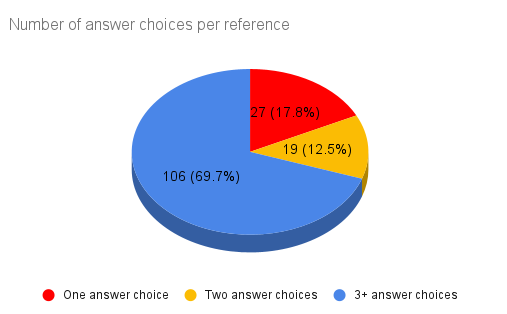
\includegraphics[scale=0.5]{images/AnswerRef.png}
\caption{The color questions in the training data sorted by textual reference. In total we find in all color questions 153 references. 17.8 percent of the references have one color answer as the only choice.  }
\label{fig:AnswerRef}
\end{figure}.

We find that 17.8 percent of the references have one color answer as the only choice of answer, as seen in figure \ref{fig:AnswerRef}. This means that 17.8 percent, 1755 of allthe  9861 "color" \& "color\_room" QA episodes in the train-set, have one possible color as an answer. This means, in these cases the model does not train on disambiguating any classes of color for the reference in the question. These data sample would instead tell the model that there is only one possible answer to memorise for this reference. (Appendices contain all the textual references found in the question)

Second type of bias is the dominance of one color over the other choices in the question-answers with multiple color choices. (visualization to be added)



\subsubsection{Navigation Model}


Habitat's navigation is referred to as PACMAN. It consist of two core components, planner and controller. The planner takes inputs from the vision and language model, and the encoding of hidden-layer and action of the previous time-step , then outputs action-decision. 

\begin{figure}[H]
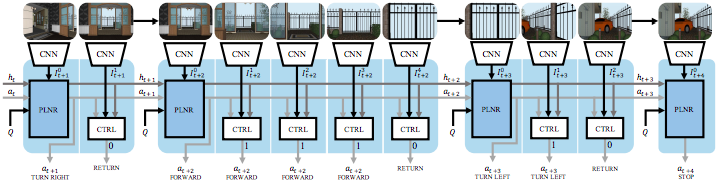
\includegraphics[scale=0.53]{images/nav.png}
\caption{}
\label{fig:nav}
\end{figure}

The controller takes the previous hidden state and action-decision and executes the action. As seen in \ref{fig:nav}, visual input is passed to the control then the controller classify the next decision of two possible decisions. Either to repeat the last action given by the planner or to return to the planner. The controller can repeat the same action maximum five times then it automatically returns to the planner. 

Visualization of the navigation is in figure (1). T stands for the planner's time-steps, t = 1,2,3...., and N(t),  n = 0,1,2,3.. denotes the controllers time-steps. The denotations of symbols explained clearer in the quotation : 


"\begin{math}  I_{t}^{n} \end{math}denote the encoding of the observed image at t-th planner-time and n-th controller-time. The planner is instantiated as an LSTM. Thus, it maintains a hidden state \begin{math} h^{t}\end{math}
(updated only at planner timesteps), and samples action 
\begin{math}  a_{t} \ \in \ \{forward,\ turn-left,\ turn-right,\ stop\} \end{math} "p(6)
\vspace{0.3cm}

For eample the first  step-decesion from the planner is denoted as such: 
\vspace{0.3cm}

\hspace{1cm}        \begin{math} a_{t} ,h_{t}{}\leftarrow PLNR\left( h_{t-1} ,I_{t}^{o} ,Q,a_{t-1}\right) \end{math},
        
\vspace{0.3cm}

The planner computes the next step-action  \begin{math} a_{t+1} \end{math} from input of the previous hidden layer \begin{math} (h_{t-1}) \end{math}, question encoding (Q), the previous action  \begin{math} a_{t-1} \end{math}, and the image input given to the PlNR \begin{math} (tI_{t}^{o}) \end{math}.The planner selects the action \begin{math} a_{t+1}\end{math} and update the hidden state \begin{math} h_{t+1} \end{math} then passes the control to the controller. 

\vspace{0.3cm}


The controller decides to either repeat the action or return control to the planner. The controller's classification is based on the current hidden-state\begin{math} h_{t}  \end{math} and current action \begin{math} a_{t} \end{math} and the image observation from the planner + the image given at the controller's time-step. The denotation of the classification is as such: 

\vspace{0.3cm}

\[ \{0,1\} \ \backepsilon \ c_{n}^{t} \ \leftarrow CTRL\ \left( h_{t} ,a_{t} ,I_{t}^{n}\right)  \]

"if \begin{math} c_{n}^{t} = 1 \end{math} then the action \begin{math} a_{t} \end{math} repeats. Else \begin{math} c_{n}^{t} = 0 \end{math} or a max of 5 controller-times been reached, control is returned to the planner"p(6). The \begin{math} h_{t} \end{math}   \begin{math} a_{t} \end{math} coming from the planner act as an intent. The controller, initiated  as "feed-forward multi-layer perceptron with 1 hidden layer",repeats and controls the action in order to align \begin{math}  I_{t}^{n} \end{math} with intent given by the planner. 

\subsubsection{VQA Model}



The VQA model is a CNN-LSTM architecture.The CNN encodes a 224x224 RGB images with a “multi-task pixel-to-pixel prediction framework”(p6) encoding. The structure of the CNN4 {5x5 Conv, BatchNorm, ReLU, 2x2 Max-Pool blocks}, and they produce a fixed-size representation.“The range of depth values for every pixel lies in the range r0, 1s, and the segmentation is done over 191 classes”(p.11) \cite{embodiedqa} . The lstm is a 2-layer LSTM with 128d hidden layers





\begin{figure}[H]
\centering
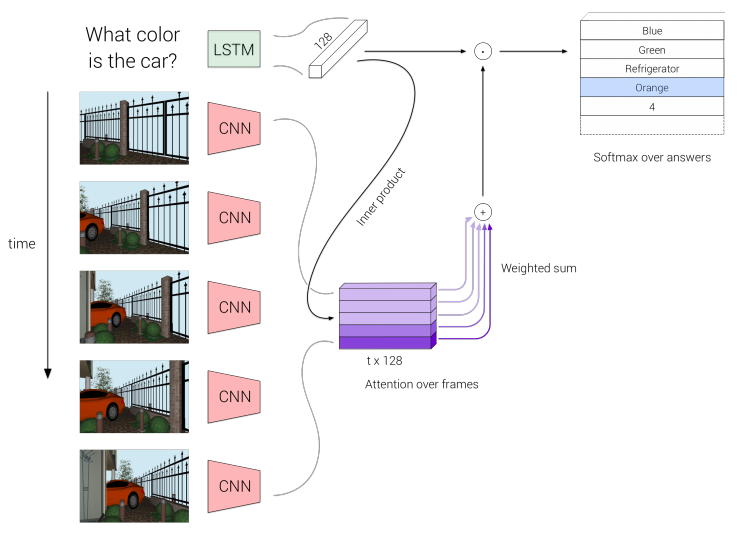
\includegraphics[scale=0.35]{images/VQA.png}
\caption{Architecture of the VQA model consist of and LSTM for language encoding, CNN for vision. The system is trained to combine the two with attention}
\label{fig:VQ}
\end{figure}



The CNN extracts features from five images(5 frames) scene, and the LSTM encodes the textual features of the question. Combing the visual and linguistic features is done through computing similarity via dot product and concatenation. First the similarity between each image and the question features is computed via dot product. A soft max converts the question and image similarity into attention wights then the question encoding is concatenated with them. The concatenated features are then classified in a soft max, where the answer probability is distributed over 172 answers.(\cite{embodiedqa},p6)



\subsection{Problem}

In an experiment we conducted on the VQA model, we observed that the system tends to answer the questions relying mainly on the textual input in the questions (bias)\footnote{ Link to the experiment "Testing VQA's reliance on vision "  \url{https://github.com/Al-arug/Habitat-Project}.} The idea of the experiment was to give the model a random image instead of the original scene and see if it affects its predictions. The results showed that the system gave correct answers despite the absence of the corresponding scene required to answer the question. In such a case, the system's performance, would normally, have worsened not improved as the required visual information to answer the question is missing. The correct answering by the system was demonstrated in an overall increase in the performance score. Its ability to answer correctly demonstrates its reliance on the language model to predict the answer. 

The system's ability to predict answers correctly in the experiment indicates lack of visual grounding. We draw this conclusion from the observation that vision had no influence on the predictions. This means that the system, in the training, has not learnt a scheme for word-meaning in association to vision. Grounding language in vision is when we connect the "high-level" symbolic representations such language to a "low-level" non-symbolic representation such as the sensory (visual) features. The ability to ground language in vision is important for any task requiring "seeing" and attending answer. If a robot successfully learns to align and combine the two types of representations, one could say that the computer understands what it sees (visual grounding). When a system fails to achieve such a connection, we define the problem as the  "Symbol system problem"(\cite{harnad1990symbol}) or 'lack of visual grounding' 


We presume that the lack of visual grounding  is attributed to bias in the data-set. Earlier in this text we reviewed textual biases within the EQA data-set. Having biases in the data-set would hinder the learning process, as it gives the model a way to learn to avoid combining vision and language  by giving  correct answers without actually learning to combine the two types of data. 

We also observe that the type of questions asked are simplistic and can be considered unnatural. The existent color questions in the data-set are not the type of questions that a human would naturally ask. The limited types of questions found in the data-set seems to be meant for simplifying the task on the robot with a main focus on navigation.


\subsection{Problem in a context}

(\cite{selvaraju2020squinting},\cite {goyal2017making}) and other research within the VQA point out the problem where  models learn biases in training and manage to give good results in the testing.\cite{johnson2017clevr} elaborate that the underlying issue here is that the model answers by memorising prior textual information. For example, a neural network might answer the question “What covers the ground?” correctly by answering “snow”, “not because it understands the scene but because biased data-sets often ask questions about the ground when it is snow-covered.” \cite{fukui2016multimodal} clarify that the models' answer-cheating is demonstrated when a VQA system primarily relies on the language model , and ignores the visual information. Such a learning problem is crucial because it makes it challenging to evaluate the model’s improvements\cite{agrawal2018don}.

When a system cheats its way into answering the questions it shows lack of visual grounding\cite {goyal2017making}. Visual grounding (understanding the meaning of words in reference to vision)is important because we want the systems to understand the reasoning steps that humans would logically take to answer a question \cite{agrawal2016analyzing},\cite{zhang2016yin}, \cite {fukui2016multimodal}. For the systems to be able to reason its way to predict an answer it must first capture the full meaning. \cite{selvaraju2020squinting} explains that learning to reason would require the systems to make inferences at "multiple levels of abstraction". For example, "is the banana ripe?" where it would instantly answer "no".  To answer this question, it would require the system to rely on perception to answer sub-questions such as where is the object? What are its shape, size, and color? Then reason that the "yellow" color indicates ripeness.\cite{selvaraju2020squinting}

\subsection{Research Questions}
\begin{itemize}


\item How can we extend the data-set with more sophisticated and natural questions ? (A useful robot should answer a variety of questions.)

Adding new questions could help test the system's capabilities, but more importantly, we consider it a step to enhance the system's cognition. The VQA system that we are improving is part of a robotic system that should ideally be helpful for human use. Social robot's usability is very dependent on its exhibition of human intelligence \cite{fong2003survey}.

\item How does the VQA system preform with the new question types ? 

\item Does asking questions of spatial and size types improve the system's attention to vision ? (Evaluating it based on the performance on color questions) 


\end{itemize}

 

